\section{Scalable Kd-tree Partitioner with Dangle and Cut Edges Integration} \label{sec:extension_methods}

\subsubsection{Kd-tree Partition Strategy} %\label{sec:kdtreestrategy}
In Section \ref{sec:pstrategies}, we use the quadtree spatial index as the baseline for our partitioning strategy. The quadtree follows a space-oriented approach, as it does not consider the content of each cell when determining potential splits. In contrast, kd-tree-based partitioning employs a data-oriented approach by sorting and selecting the midpoint within a cell to guide the placement of splits for future child nodes.

Building and populating the kd-tree partitioning follows a process similar to that of the quadtree. First, a kd-tree is constructed from a sample representing 1\% of the input data to define the tree’s structure, where the leaves represent the partition’s cells. The input data is then fed into this kd-tree structure, with each edge assigned to the leaf cell containing its boundaries. After partitioning, the local DCELs for each layer are constructed, and the overlay operation is performed within each cell as described in Section \ref{sec:pstrategies}.

Section \ref{sec:extension_experiments} will compare two partitioning strategies, the one presented in \ref{sec:pstrategies} based on the quadtree (i.e. space-oriented) and one on the kd-tree (i.e. data-oriented) indexes.  Note that both tree-based data partitioning involves shuffling all edges; this however, happens only once. Our experimental evaluation (see Section \ref{sec:comparison}) shows that the data-oriented approach leads to better performance. 

\subsection{Overlaying Polygons with Dangle and Cut Edges} \label{sec:over_dang}

Beyond scalability challenges, many modern applications receive spatial polygon datasets as scattered line segments—for example, road segments that form city blocks. Such datasets can be extremely large and are common in fields like urban planning, geo-targeted advertising, economic and demographic studies, and more. However, existing polygon overlay techniques are not equipped to process them directly at scale. In this section, we extend the overlay method presented in Section \ref{sec:methods} to support polygonal input by integrating a scalable, distributed polygon extraction approach. This enhancement enables the merging of polygons with dangle and cut edges.

We built on in the scalable polygonization procedure presented in \cite{abdelhafeez_ddcel_2023}.  The result of that polygonization procedure generates two outputs: first, a set of closed polygons formed by the input planar line segments, and second, any edges that are not a part of any polygon (i.e., dangle or cut edges).  Overlaying the polygons generated with any polygon layer follows the approaches discussed in sections \ref{sec:methods} and \ref{sec:alternative_methods}.  However, we need to modify the algorithms provided in these previous sections to overlay an input polygon layer $A$ with the dangle and cut edges (layer $B$). In particular, we modify the reduce phase.

We build upon the scalable polygonization procedure presented in \cite{abdelhafeez_ddcel_2023} (see Figure \ref{fig:polygonization}), which produces two outputs: (1) a set of closed polygons formed from the input planar line segments, and (2) any edges that are not part of any polygon (i.e., dangle or cut edges). Overlaying these generated polygons with any polygon layer follows the methods discussed in Sections \ref{sec:methods} and \ref{sec:alternative_methods}. However, to overlay an input polygon layer $A$ with the dangle and cut edges (layer $B$), we modify the algorithms from these sections, particularly adjusting the reduce phase.

 \begin{figure}
     \centering
     \begin{tabular}{cc}
         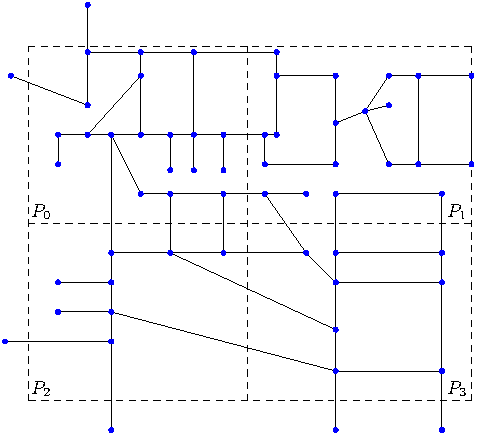
\includegraphics[width=0.49\textwidth]{chapterExtension/model/input/input} &
         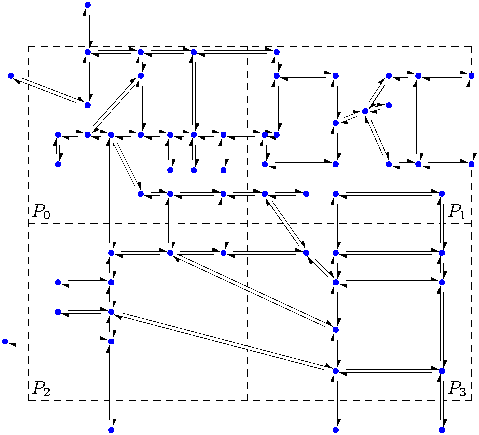
\includegraphics[width=0.49\textwidth]{chapterExtension/model/a/a} \\
         (a) & (b) \\
         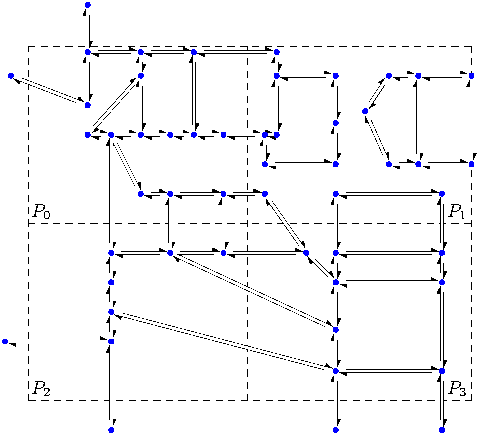
\includegraphics[width=0.49\textwidth]{chapterExtension/model/b/b} &
         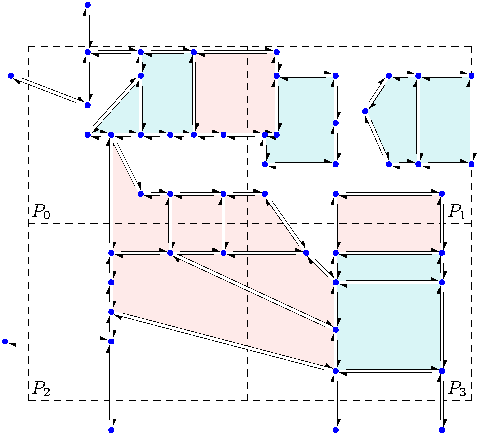
\includegraphics[width=0.49\textwidth]{chapterExtension/model/c/c} \\
         (c) & (d) \\
     \end{tabular}
     \caption{An example of four leaf nodes in a quadtree constructed for input spatial line segments. Solid lines represent the line segments, while dashed lines indicate the Minimum Bounding Rectangles (MBRs) of the partitions. (a) shows the partitioned input spatial lines. (b) shows the DCEL vertices and half-edges. (c) the resulting DCEL after  dangle and cut edge removal.  Finally, (d) shows the final DCEL faces. (taken from \cite{abdelhafeez_ddcel_2023}).} \label{fig:polygonization}
 \end{figure}

 \begin{figure}
    \centering
    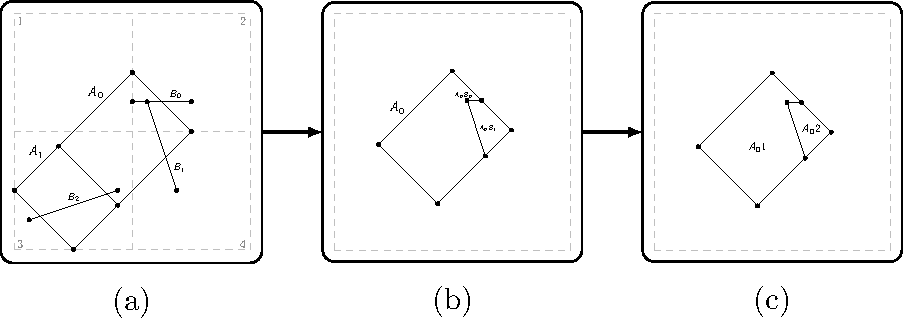
\includegraphics[width=\textwidth]{chapterExtension/dangles_cuts/DAC}
    \caption{(a) Spatial partitioning of input layers A and B, (b) Re-Partitioning of polygon $A_0$ with edges it intersects with, and (c) the result of polygonization of $A_0$ with $B_0, B_1, B_2$.} \label{fig:dangles_cuts}
 \end{figure}

 Figure \ref{fig:dangles_cuts}(a) illustrates the spatial partitioning of two input layers, $A$ and $B$. Layer $A$ contains two input polygons, $A_0$ and $A_1$, while Layer $B$ includes of three dangle edges, $B_0$, $B_1$, and $B_2$.
 
 Each edge in layer $B$ is assigned a unique label and provided as input to the overlay module.  The local overlay processs indentifies intersections between the input polygon layer $A$ and layer $B$ within each data partition.  If a polygon with $id = i$ from layer $A$ intersects with edges labeled $id = a$, $id = b$ and $id = c$ from layer $B$ in a given partition, a composite label $A_{i} B_{a} B_{b} B_{c}$ is generated to represent these intersections.  
 
During the reduce phase, we re-partition the data based on the first label, consolidating all edges that intersect with it. For instance, if two data partitions generate the labels $A_{i} B_{a} B_{b} B_{c}$ and $A_{i} B_{x} B_{y}$, we reassign the data so that $A_{i}$ is grouped within a single partition along with all intersecting edges, specifically $B_{a}, B_{b}, B_{c}, B_{x}, B_{y}$.  In Figure \ref{fig:dangles_cuts}(b), polygon $A_0$ is re-partitioned with the edges it intersects, namely $B_0$, $B_1$, and $B_2$.

After re-partitioning, all intersecting edges from both layers are consolidated within the same partition. The next step is to identify the polygons formed by these intersections. Since there is no guarantee that only one polygon will be generated, we replace the polygon concatenation method proposed in Section \ref{sec:optimizing} with a \textit{polygonization} procedure within each partition. This polygonization process ensures that all possible new polygons are generated.

The polygonization procedure follows the algorithm outlined in \cite{abdelhafeez_ddcel_2023}. It begins by generating new vertices and half-edges, marking the current dangle and cut edges, setting the next pointers, and finally constructing the partition polygons. Figure \ref{fig:dangles_cuts}(c) illustrates the result of polygonizing the edges from polygon$A_0$ and $B_0$, $B_1$, and $B_2$, yielding two polygons,$A_01$ and $A_02$.  The polygons generated from all partitions together form the overlay between polygon layer $A$ and layer $B$.
